\documentclass[tikz,border=2pt]{standalone}
\usepackage{amsmath}
\usepackage{pgfplots}
\pgfplotsset{compat=1.18}
\usetikzlibrary{arrows.meta}
\begin{document}
% Left (Example 1): min x1^2+x2^2 s.t. x1+x2>=1 -- convex halfplane, level circles Z=1/2 and Z=1, unique optimum (1/2,1/2), Z=1/2.
% Right (Example 3): min 3x^2 on [-2,1]u[2,3] (nonconvex constraint) -- local minimum x=2 (Z=12), global minimum x=0 (Z=0).
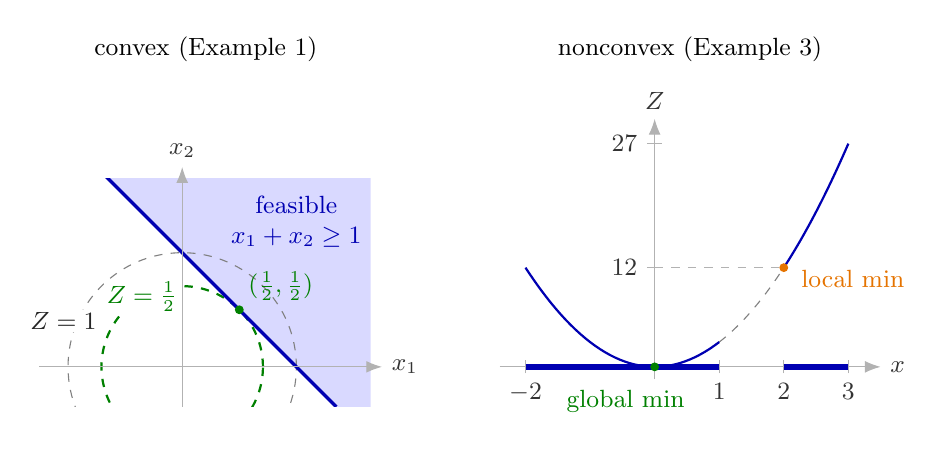
\begin{tikzpicture}[font=\small, >={Latex[length=2mm]}]
  % ---------------- left panel: convex problem ----------------
  \begin{scope}[x=1.45cm, y=1.45cm]
    \begin{scope}
      \clip (-1.25,-0.35) rectangle (1.65,1.65);
      \fill[blue!15] (-0.85,1.85) -- (1.65,1.85) -- (1.65,-0.35) -- (1.35,-0.35) -- cycle;
      \draw[gray, dashed] (0,0) circle (1);
      \draw[green!50!black, thick, dashed] (0,0) circle ({sqrt(0.5)});
      \draw[blue!70!black, very thick] (-0.85,1.85) -- (1.35,-0.35);
    \end{scope}
    \draw[gray!60, ->] (-1.25,0) -- (1.75,0) node[anchor=west, gray!40!black] {$x_1$};
    \draw[gray!60, ->] (0,-0.35) -- (0,1.75) node[anchor=south, gray!40!black] {$x_2$};
    \node[blue!70!black, align=center] at (1.0,1.27) {feasible\\$x_1+x_2\geq1$};
    \node[green!50!black, fill=white, inner sep=1pt] at ({cos(120)*sqrt(0.5)},{sin(120)*sqrt(0.5)}) {$Z=\tfrac{1}{2}$};
    \node[gray!30!black, fill=white, inner sep=1pt] at ({cos(160)-0.1},{sin(160)+0.06}) {$Z=1$};
    \fill[green!50!black] (0.5,0.5) circle (1.6pt);
    \node[green!50!black, anchor=south west, inner sep=1pt] at (0.55,0.55) {$(\tfrac{1}{2},\tfrac{1}{2})$};
  \end{scope}
  \node[anchor=south] at (0.3cm,3.75cm) {convex (Example 1)};
  % ---------------- right panel: nonconvex constraint ----------------
  \begin{scope}[xshift=6.0cm, x=0.82cm, y=0.105cm]
    \draw[gray!60, ->] (-2.4,0) -- (3.5,0) node[anchor=west, gray!40!black] {$x$};
    \draw[gray!60, ->] (0,-1.5) -- (0,30) node[anchor=south, gray!40!black] {$Z$};
    \foreach \t in {-2,1,2,3} \draw[gray!60] (\t,-0.8) -- (\t,0.8) node[at start, anchor=north, gray!40!black] {$\t$};
    \draw[gray!60] (-0.12,12) -- (0.12,12) node[at start, anchor=east, gray!40!black] {$12$};
    \draw[gray!60] (-0.12,27) -- (0.12,27) node[at start, anchor=east, gray!40!black] {$27$};
    % objective on the gap (infeasible) and on the feasible pieces
    \draw[gray, dashed, domain=1:2, samples=20] plot (\x,{3*\x*\x});
    \draw[blue!70!black, thick, domain=-2:1, samples=40] plot (\x,{3*\x*\x});
    \draw[blue!70!black, thick, domain=2:3, samples=20] plot (\x,{3*\x*\x});
    % feasible region [-2,1] u [2,3] on the axis
    \draw[blue!70!black, line width=2.2pt] (-2,0) -- (1,0);
    \draw[blue!70!black, line width=2.2pt] (2,0) -- (3,0);
    \draw[gray!60, dashed] (0,12) -- (2,12);
    \fill[orange!90!black] (2,12) circle (1.6pt);
    \node[orange!90!black, anchor=west] at (2.12,10.6) {local min};
    \fill[green!50!black] (0,0) circle (1.6pt);
    \node[green!50!black, anchor=north] at (-0.45,-1.6) {global min};
  \end{scope}
  \node[anchor=south] at (6.45cm,3.75cm) {nonconvex (Example 3)};
\end{tikzpicture}
\end{document}
